% 2020 江苏卷 13：△ABC 中 D 在边 BC 上，延长 AD 到 P（AP=9）
% 绘制依据：固定源 PDF 第 1115 面原图。A 左下、B 右下、C 左上（∠BAC=90°），
% D 在 BC 上，连 PA、PB、PC（P 在右方远处）。只标 A、B、C、D、P 五点。
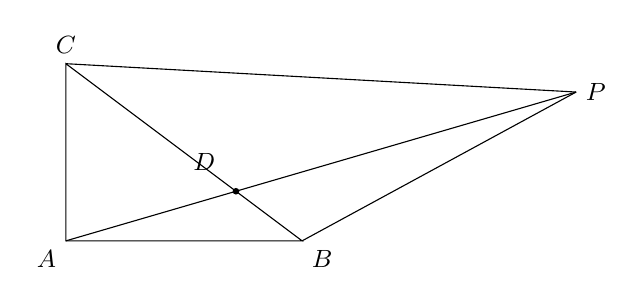
\begin{tikzpicture}[scale=0.75, font=\small]
  \coordinate (A) at (0,0);
  \coordinate (B) at (4,0);
  \coordinate (C) at (0,3);
  \coordinate (D) at (2.88,0.84);
  \coordinate (P) at (8.64,2.52);
  \draw (A) -- (B) -- (C) -- cycle;
  \draw (A) -- (P);
  \draw (B) -- (P);
  \draw (C) -- (P);
  \fill (D) circle (1.6pt);
  \node[below left] at (A) {$A$};
  \node[below right] at (B) {$B$};
  \node[above] at (C) {$C$};
  \node[above left=4pt] at (D) {$D$};
  \node[right] at (P) {$P$};
\end{tikzpicture}
